%======================================================================
\subsection{BW-ROU-08 --- Built, 30 Oct: flexible wires that keep their length}\label{sec:rou-flex-built}
%======================================================================

Built the same evening in four commits: the solver \code{da6873a6}, wires as ropes \code{7ff9ecaf}, the Assembly
hook \code{454fa6ff}, robustness and the battery tests \code{5c308923} (plus a last fix for proxies,
see below). Following the brief to keep it lean: collision proxies are \emph{oriented boxes only}, the stiffness
table has PVC and silicone, the panels got one field and one status line.

\begin{figure}[!htbp]
\centering
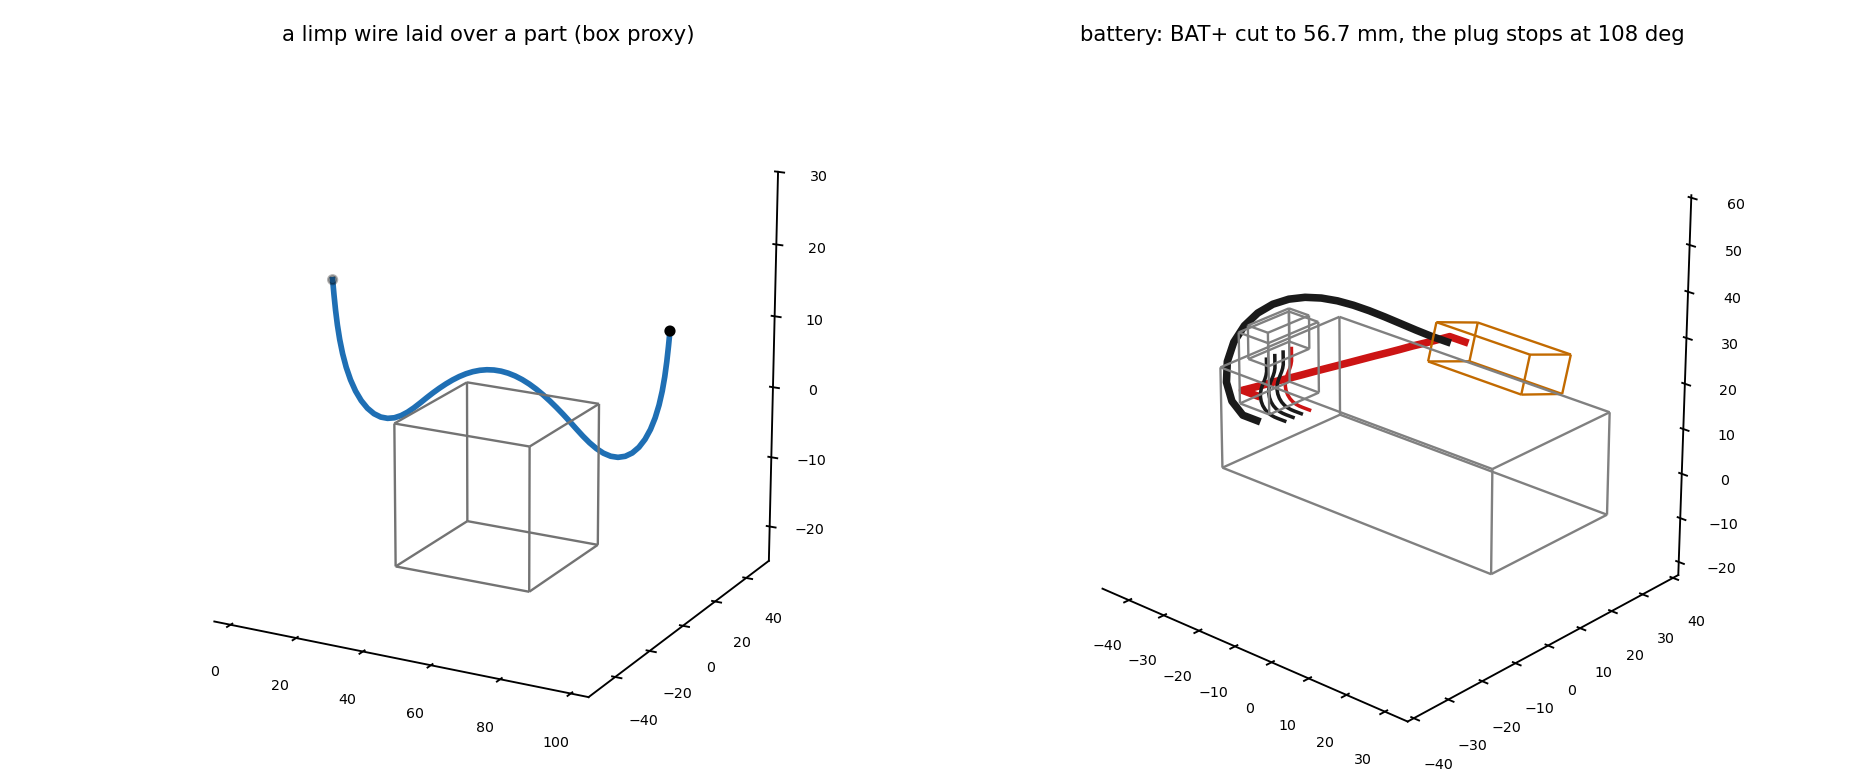
\includegraphics[width=\linewidth]{fig/rouflex_battery.png}
\caption{Left: a limp wire (EI $20$\,N\,mm$^2$) 116\,mm long between two points 100\,mm apart, laid over a box
proxy; no point is inside it and the surplus length arches above. Right: the battery \code{STD-02-01001-001} (vault
copy), the T plug hinged on the pack and swung with the Assembly drag API, BAT$+$ cut to 56.7\,mm: the drag stops at
108$^\circ$ of the 180$^\circ$ asked, the red lead is just taut. Both are plots of the real rope states (matplotlib,
not the 3D view).}
\label{fig:rou-flex-built}
\end{figure}

\paragraph{What you can do now.}
\begin{itemize}[nosep]
  \item \textbf{Every wire, hose and bundle is a rope} (pipes stay rigid). \code{CutLength} is the item's own length,
        any value; nothing stretches. Existing items took their present length with slack (W2); \code{Slack} now edits
        the cut length. The route path only gives the first layout. A hidden \code{RopePoints} holds the shape, so a
        recompute that moves a pin solves from where the wire was.
  \item \textbf{Ends and clips.} The first and last points are the pin frames' lead straights, kept at their exact
        length. A path point attached to a part (not an end) is a clip: the wire passes through it, free to turn; a
        free-space point is only a guide.
  \item \textbf{Gravity} along $\pm X/Y/Z$ of the top assembly: property \code{BWGravity} (made when a wire is
        made), default $-Z$, fallback preference \code{Mod/BruceWorx/Routing/Gravity}.
  \item \textbf{Taut or too bent} (outside a drag): red, Browser badge ``taut'', \code{Problems} text, the panel's
        status line (``taut'' or ``sagging, N\,mm below the straight line'').
  \item \textbf{Live drag.} \code{AssemblyObject} calls \code{bruceworx\_drag.pre\_drag / check / post\_drag} ($[BW]$ in
        \code{validateNewPlacements}). \code{check} solves the wires on the moved parts at the proposed pin
        positions, warm-started; a step that makes a wire more taut or more bent than where the drag began is
        refused, through the same bisection as a joint limit. While dragging the wires are drawn as Coin line sets (their
        colour, width from the OD) in place of the solids; the solid is rebuilt on release.
  \item \textbf{Panels} (Wire, Hose): a \emph{Cut length} field and the status line. \code{StiffnessFactor} is a
        property (no hang-test dialog).
\end{itemize}

\paragraph{Benchmarks} (\file{addons/BruceWorx/tests/test\_rope.py}, 9 tests; run with the pixi Python, which has numpy).
\begin{center}\small
\begin{tabularx}{\linewidth}{@{}lXl@{}}
\toprule
Test & Result & Limit \\
\midrule
Catenary $d=200$, $L=250$, $EI\to0$ & $a=84.55$; sag 66.364 vs 66.359\,mm (0.007\,\%) & 1\,\% \\
12\,AWG stub 100\,mm & $EI=1691$\,N\,mm$^2$, $q=3.853\times10^{-4}$\,N/mm, tip sag 2.797 vs $qL^4/8EI=2.848$\,mm (1.8\,\%) & 5\,\% \\
Length after 25 random end moves & within $10^{-3}$ & $10^{-3}$ \\
Bend limit, pin turned back & turning ratio $0.98$ of the limit & $\le1$ \\
Box collision & no point inside; resting points at the wire radius & $10^{-2}$\,mm \\
Taut detection & 300\,mm apart with $L=250$ taut; 200\,mm free & --- \\
6 wires $\times$ 40 points, warm start & 2.0\,ms per drag step (3 outer steps) & 10\,ms \\
\bottomrule
\end{tabularx}
\end{center}
The tables: $EI=E_{\rm Cu}\,n_s\pi d_s^4/64+E_i\pi(D^4-d^4)/64$ with $E_{\rm Cu}=117$\,GPa, 65 strands of 0.254\,mm for
12\,AWG (1554) and PVC $E=18.6$\,MPa (137); silicone 5\,MPa. $q=(\rho_{\rm Cu}A_c+\rho_iA_i)g$ is
$3.85\times10^{-4}$\,N/mm for 12\,AWG (the plan's $3.74\times10^{-4}$ used a thinner wall; the test recomputes the
expected sag from the tables). One point per 1.5\,OD, 20--200.

\paragraph{Battery} (a copy of the vault, \file{TestBruceWorxRopeCore.BatteryTests}, set \code{BW\_BATTERY}; hinge
joint added on the pack's \code{LeadEnd} and the plug's \code{MateFace}): six wires through a 47-step arc and back keep
their lengths exactly (rope length $=$ cut length), 2.8\,ms per step without proxies and 14\,ms with the box proxies
of the pack, the balance plug and its cover (about 70 steps/s); with BAT$+$ shortened to 56.7\,mm the plug stops at
107.7$^\circ$. The Assembly tests (\code{TestBWJoints} 13, motion 16, workbench 44), the routing core (30), the new
rope core (8) and the Routing GUI suite (13) pass.

\paragraph{Decided while building.}
\begin{itemize}[nosep]
  \item \textbf{Solver.} Not Gauss--Seidel: a gravity step made first-order compatible with the constraints, then a
        global Newton solve of all lengths and bendings (bending as a smooth vector constraint $x_{i-1}-2x_i+x_{i+1}$,
        eliminated exactly, one $(N-1)^2$ system per wire). Position-based sweeps could not hold a hanging rope (they
        stretch), and a scalar $|d|$ bending constraint lets out-of-plane loads through. Equilibrium does not depend on the
        step size, so a drag step starts from the last shape and needs three outer steps.
  \item \textbf{A limit that cannot be met.} The hard bend-limit rows can over-determine a node. The solver tightens
        the limit gradually from an over-bent layout and, if the hard rows fail, retries with the limit as a stiff
        spring and keeps the better result: an infeasible wire stays finite and red instead of blowing up.
  \item \textbf{The battery as built is infeasible.} Its leads bend tighter than the silicone 3\,$\times$\,OD rule
        (BAT$+$: 4.3 against 10.8\,mm; the old model already said \code{BendOK} false). It now shows red; a drag refuses
        a step only if it makes things worse than where it began, so such a wire is not frozen. The tests set the rule
        to ``No check'' for the arc.
  \item \textbf{Proxies.} A part whose box already holds an end of the wire (the clear cover over the balance plug) is
        no obstacle to it; the parts the ends sit on are skipped. A point inside a box leaves against gravity, so a wire
        falling into a part ends up draped over it.
  \item \textbf{Old tests changed.} Tests that expected the wire to follow the path (length $=$ path\,$\times$\,1.05 after a
        pin changed, a bend flag from a tight path corner) now expect the rope: the cut length is the wire's own, and a
        rope relaxes a path's tight corner. Tight-bend cases use a cut length too short for the radius.
\end{itemize}

\paragraph{Open questions for you.}
\begin{enumerate}[nosep]
  \item \textbf{Unconnected parts.} A part with no joint (the battery's plug as built) is moved by the 3D view directly
        and is not in the drag solve, so the stop cannot cut its move back. Hinge or slide it to make it stoppable, or
        also back off unconnected parts?
  \item \textbf{Bundles} are one rope with the wires' summed stiffness; the wires inside still have their own ropes, so
        they do not follow the bundle's shape. Make member wires copy the bundle's shape?
  \item \textbf{Not built (kept lean):} convex hull / mesh proxies per part (a TODO in \file{bruceworx\_rope.py}), the hang-test
        calibration dialog, wire-to-wire contact, flexible sub-assemblies carrying routed items (agent \code{flexsub}), a
        command for the gravity axis (it is a property on the assembly).
  \item \textbf{Cost with proxies} is 14\,ms per step for the battery; box tests are plain numpy. A broad phase would bring it
        back to 3\,ms. Worth doing before big assemblies?
\end{enumerate}

\paragraph{Answers (30 Oct).} Parts without a joint: add a joint (hinge or slider) to get the drag stop; no
change to the drag. Wires inside a bundle follow the bundle's rope shape: next round. 14\,ms per drag step with
proxies is fine; a broad phase waits for larger assemblies.

\paragraph{Gravity toggle (31 Oct).} Gravity is \emph{off} by default (the user's call, so no sag work is done unless
asked for); a bool \code{BWGravityOn} on the top assembly, beside the axis \code{BWGravity}, switches it, and an
assembly saved before the switch reads as off. Off, a rope keeps its cut length, bend limit and contacts (the solver
skips only the gravity step; the push-out direction of a contact is still the gravity axis) and the status reads
``slack, gravity off''. The switch is the Gravity button in the Routing tab's Items group (shows on/off), a small
button on the 3D view's navigation pill (lit when on, shown only while the active assembly has flexible wires) and the
shortcut G, V (free: Draft uses G, R and Sketcher G, A/L/M/Y). It acts on the selected wire's assembly, else the active
assembly, else the document's only assembly with wires, and recomputes its wires once. Cost: a rope is re-solved only
when something it depends on changes. FreeCAD recomputes only touched objects and the rope code has no timers or
observers of its own, so nothing re-solves while idle; in addition a wire touched through a dependency now compares a
signature (ends, clips, cut length, mechanics, gravity direction and on/off, proxy boxes near it) and keeps its solved
shape when nothing it depends on moved. Tests: a wire between level pins with gravity off has no sag and the same
length, a second recompute makes no solver call, switching on solves once.

\paragraph{31 Oct follow-ups.} The wires of a bundle now take their centreline from the bundle's solved rope: after the
bundle solves (a recompute or a drag) each member wire is redrawn through the bundle's points and keeps its own cut
length, with no separate solve; during a drag only the bundle is solved. Bundles have no breakouts yet, so a wire follows
the bundle between its ends (leads outside the span come with breakouts). The Wire, Pipe, Hose and Route Path commands
refuse a flexible sub-assembly copy (an object with \code{FlexSource}): the panel does not open and the status bar shows
``Edit this wire in its sub-assembly''. Tests: a bundle of three wires after a drag step (centrelines within OD/2 of the
bundle's, cut lengths unchanged) and a command on a copy opening no panel.
